\documentclass[11pt]{article}
\usepackage[a4paper,margin=2.5cm]{geometry}
\usepackage[T1]{fontenc}
\usepackage[utf8]{inputenc}
\usepackage{amsmath,amssymb}
\usepackage{booktabs,array}
\usepackage{graphicx}
\usepackage{xcolor}
\usepackage[numbers,sort&compress]{natbib}
\usepackage[colorlinks=true,linkcolor=blue!50!black,citecolor=blue!50!black,urlcolor=blue!50!black]{hyperref}
\graphicspath{{../leakage/}}

\newcommand{\qgZ}{qg_Z}

\title{¿Cuándo ayuda leer el tercer nivel?\\
Marcas de fuga, qubits de borrado y el decodificador qg sensible a T1}
\author{Vicente Humberto Monteverde\\
\small Universidad del Museo Social Argentino (UMSA), Argentina\\
\small ORCID 0000-0001-8884-4811}
\date{\small Borrador del 29 de septiembre de 2026 (traducción de la versión en inglés)}

\renewcommand{\abstractname}{Resumen}
\renewcommand{\tablename}{Tabla}
\renewcommand{\figurename}{Figura}
\renewcommand{\refname}{Referencias}

\begin{document}
\maketitle

\begin{abstract}
Los qubits transmón se fugan a su segundo estado excitado, y una lectura de tres niveles puede
marcarlo. Nos preguntamos si esto ayuda al decodificador qg sensible a T1, un decodificador de
emparejamiento de peso mínimo cuyos pesos siguen la lectura final de los datos y que un testigo de
sesgo polar promediado sobre el registro activa solo cuando domina la
relajación~\cite{monteverde2026qang,monteverde2026witness}. Seis pruebas simuladas sobre una memoria
de código de superficie con ruido de circuito, cada una con su criterio fijado antes de la corrida
reportada, dan una respuesta coherente. (i) Cuando un qubit fugado conserva su valor, borrar los qubits
marcados empeora todos los decodificadores, y toda la ganancia de qg (1{,}68$\times$) viene de la
reponderación a nivel de qubit. (ii) Cuando la fuga desordena el valor, la marca y la reponderación
combinadas rinden más que cada una por separado: 1{,}68$\times$ sobre el mejor decodificador con
manejo de fuga a distancia 3. (iii) Un peso bayesiano para la marca, una probabilidad de inversión
$a/(1+a)$ con $a$ la asimetría de fuga entre $|0\rangle$ y $|1\rangle$, contiene ambos casos, nunca es
peor que ignorar la fuga y no es uniformemente mejor que el borrado (una de cuatro predicciones
falla). La ganancia combinada crece con la distancia, de 1{,}48$\times$ a 1{,}77$\times$. (iv) Una
simulación coherente de tres niveles de una CZ diabática da $a=0$ y un qubit fugado que conserva su
valor y sigue invirtiendo su ancilla con probabilidad 0{,}97. Para esos transmones la marca es inútil,
el borrado perjudica y la ganancia de qg (1{,}81$\times$ a $d=3$, 2{,}02$\times$ a $d=5$) no necesita
lectura de qutrit. (v) En qubits de borrado, que anuncian los decaimientos T1 en el momento en que
ocurren, combinar qg de forma ingenua perjudica cuando el anuncio es bueno (0{,}46$\times$ con
eficiencia de anuncio $h=0{,}99$); escalar la probabilidad previa de los decaimientos no anunciados
por $1-h$, una regla puesta a prueba después con su propio registro previo, elimina la pérdida y
conserva una ganancia de 1{,}41--1{,}68$\times$ con $h=0{,}5$. Todos los resultados son simulaciones, reproducidas por scripts y fijadas por
tests de regresión.
\end{abstract}

\section{La pregunta}

La unidad qg describe un qubit por su sesgo polar $\qgZ=\langle\sigma_z\rangle$ y cantidades
relacionadas~\cite{monteverde2026qang}. En una memoria de código de superficie, la relajación (T1)
sesga la lectura final de los datos hacia $0$; un preprint complementario~\cite{monteverde2026witness}
lo usa para reponderar el grafo de emparejamiento corrida por corrida (un qubit de datos leído como 1
no decayó, así que sus fallas por decaimiento se descuentan), y activa la reponderación solo cuando el
$\qgZ$ promediado sobre el registro de un lote de calibración, dividido por la tasa de detectores,
supera 1. A esto lo llamamos el decodificador qg.

Los qubits superconductores también se fugan del espacio computacional, sobre todo a $|2\rangle$, y la
fuga es una amenaza conocida para la corrección de
errores~\cite{aliferis2007leakage,suchara2015leakage,mcewen2021leakage}. Una lectura de tres niveles
puede verla, y los decodificadores con manejo de fuga tratan a los qubits marcados como
borrados~\cite{suchara2015leakage,wu2022erasure,varbanov2020leakage}. Antes de extender qang más allá
de los qubits hicimos una pregunta acotada: ¿gana algo el decodificador qg con una lectura de tres
niveles, más allá de lo que ya da el manejo estándar de la fuga? La regla acordada de antemano fue
extender qang solo si gana.

\section{Planteo}

\paragraph{Memoria y ruido.} Un código de superficie rotado en un experimento de memoria Z, distancia
$d=3$ con 3 rondas o $d=5$ con 5 rondas, simulado corrida por corrida a nivel de circuito. Ruido:
depolarizante de dos qubits $p_2$ después de cada CNOT, amortiguamiento de amplitud $\gamma$ por capa
(el doble durante la medición), inversiones de lectura $q$. Dos regímenes: dominado por T1
($p_2=0{,}0005$, $\gamma=0{,}003$, $q=0{,}002$) y depolarizante ($p_2=0{,}004$, $\gamma=0{,}0005$,
$q=0{,}002$).

\paragraph{Fuga.} Después de un CNOT un qubit de datos se fuga con probabilidad $\ell=0{,}002$ si está
en $|1\rangle$ y $a\ell$ si está en $|0\rangle$. Un control fugado golpea a su ancilla con probabilidad
$\kappa$ (1/2 salvo que se indique otra cosa), no decae y vuelve con probabilidad $r$ por capa. Tres
elecciones definen un modelo: la asimetría $a$, el valor al que vuelve (siempre $1$, o al azar) y cómo
una lectura de dos niveles asigna $|2\rangle$ (como $1$, o al azar). La lectura final de tres niveles
marca todo qubit que siga fugado.

\paragraph{Decodificadores.} Todos usan emparejamiento perfecto de peso mínimo
(PyMatching~\cite{higgott2022pymatching}) sobre el mismo grafo de detectores: \emph{estándar} (ignora
la fuga); \emph{borrado} (las aristas de lectura final de un qubit marcado reciben probabilidad $1/2$,
o, donde se indica, todas sus aristas); \emph{peso bayesiano} (Sección~\ref{sec:bayes}); \emph{qg} (la
reponderación T1); y las combinaciones qg + borrado y qg + peso bayesiano. Los decodificadores se
comparan sobre las mismas corridas con un $z$ apareado (McNemar).

\paragraph{Protocolo.} Cada prueba enuncia su criterio en el script antes de la corrida. En las cinco
últimas, el script y el criterio se subieron al repositorio público antes de la corrida reportada
(commits \texttt{3fa4d63}, \texttt{daf0b6f}, \texttt{092580f}, \texttt{e877a72},
\texttt{68d8d00}), y el código se depuró con otra semilla.

\section{Resultados}

\subsection{Un qubit fugado que conserva su valor: un resultado negativo}

En el primer modelo ($a=0$, vuelve a $1$, $|2\rangle$ leído como 1, $r=0{,}05$) comparamos qg + borrado
con borrado. El criterio (1{,}3$\times$, $z\ge3$, nunca peor) se cumplió formalmente con 1{,}65$\times$
($z=+14{,}8$), pero fue un artefacto (Tabla~\ref{tab:neg}). La referencia de borrado, que borraba toda
la historia de un qubit marcado, fue peor que ignorar la fuga en todos los regímenes ($z=-3{,}8$ a
$-6{,}0$). El decodificador qg \emph{sin} ninguna marca le ganó al estándar por 1{,}68$\times$
($z=+14{,}7$), y agregarle las marcas lo empeoró ($z$ entre $-2{,}8$ y $-4{,}9$). Borrar solo la última
capa, una variante agregada después de la primera corrida, perjudicó menos pero siguió siendo peor que
el estándar. La razón es simple: un qubit que se fuga solo desde $|1\rangle$ y vuelve a $|1\rangle$ se
lee correctamente como 1, y declararlo borrado descarta un valor correcto. Lo registramos como
resultado negativo.

\begin{table}[t]
\centering\small
\caption{Error lógico, primer modelo ($a=0$, valor conservado), $d=3$, 60\,000 corridas por régimen.}
\label{tab:neg}
\begin{tabular}{lcccc}
\toprule
régimen (testigo) & estándar & borrado & qg + borrado & qg, sin marcas\\
\midrule
fuga + dominado por T1 (1{,}68) & 0{,}0156 & 0{,}0165 & 0{,}0100 & 0{,}0093\\
fuga + mixto (1{,}27) & 0{,}0099 & 0{,}0106 & 0{,}0089 & 0{,}0084\\
fuga + depolarizante (0{,}34) & 0{,}0032 & 0{,}0036 & 0{,}0036 & 0{,}0032\\
fuga fuerte, depolarizante (0{,}46) & 0{,}0021 & 0{,}0032 & 0{,}0032 & 0{,}0021\\
\bottomrule
\end{tabular}
\end{table}

\subsection{Una fuga que desordena el valor}

Una corrida exploratoria sugirió que la marca ayuda cuando el qubit fugado pierde su valor. Entonces
fijamos un segundo modelo y un criterio más exigente antes de la corrida: fuga desde $|1\rangle$
($\ell$) y desde $|0\rangle$ ($\ell/2$), vuelta a un bit al azar, $|2\rangle$ leído al azar y marcas de
fuga en cada ronda con eficiencia 0{,}8. El criterio exigía que el decodificador qg con marcas le
ganara al \emph{mejor} de dos decodificadores con manejo de fuga por $\ge1{,}3\times$ con $z\ge3$ en
algún régimen, que nunca perdiera con $z\le-3$, y que las marcas mejoraran a qg en todos los
regímenes.

Se cumplieron ambas partes. En el régimen dominado por T1, qg + marcas llegó a 0{,}0106 contra 0{,}0177
del mejor decodificador con manejo de fuga (1{,}68$\times$, $z=+15{,}3$), y 1{,}28$\times$ en el
régimen mixto; las marcas mejoraron a qg en los cuatro regímenes ($z=+4{,}0$ a $+8{,}9$). La
combinación rinde más que el producto de sus partes: las marcas solas dieron 1{,}07$\times$ sobre el
estándar, la reponderación sola 1{,}45$\times$, juntas 1{,}78$\times$. Un mecanismo plausible es que la
reponderación confía en los bits finales de los datos, y el bit final de un qubit fugado es aleatorio,
así que borrarlo elimina un dato engañoso. Una segunda semilla dio 1{,}43$\times$ ($z=+11{,}3$). La
detección en cada ronda aportó poco a $d=3$: solo con la lectura final la ganancia fue 1{,}39$\times$.

\subsection{Una regla para la marca}\label{sec:bayes}

Los dos resultados se contradicen porque ambos borran la marca sin importar de dónde vino la fuga. Si
un qubit se fuga desde $|1\rangle$ con probabilidad $\ell$ y desde $|0\rangle$ con $a\ell$, y se lo ve en
$|2\rangle$, su valor antes de fugarse era 1 con probabilidad posterior $1/(1+a)$ (prior uniforme). El
peso bayesiano informa entonces al qubit marcado como 1 y les da a sus aristas de lectura final la
probabilidad de inversión
\begin{equation}\label{eq:pflag}
p_{\rm marca}=\max\!\left(\frac{a}{1+a},\,q\right),
\end{equation}
con un peso T1 neutro, porque un qubit fugado no decae. Con $a=0$ confía en el valor de la marca; con
$a=1$ es borrado puro. El primer modelo es el caso $a=0$, donde la regla se reduce al decodificador
estándar.

Pusimos a prueba cuatro predicciones sobre cinco modelos ($M_0$, el primer modelo; $M(a)$ con $a=0$,
$0{,}25$, $0{,}5$ o $1$, vuelta y lectura al azar; $M(0{,}5)$ es el segundo modelo), ambos regímenes a
$d=3$ y cuatro modelos a $d=5$ (Tabla~\ref{tab:bayes}, Fig.~\ref{fig:leak}). \textbf{P1} (nunca peor
que el estándar) se cumplió: $z$ entre $0{,}0$ y $+9{,}0$, mientras que el borrado perdió contra el
estándar en $M_0$ ($z=-5{,}7$). \textbf{P2} (le gana al borrado para $a\le0{,}25$ en ambos regímenes)
falló: se cumplió en el régimen dominado por T1 ($z=+6{,}1$, $+7{,}0$, $+3{,}9$) pero no en el
depolarizante ($+2{,}9$ para $M_0$, $-0{,}4$ para $M(0{,}25)$), y con $a=0{,}5$ en el depolarizante el
borrado fue apenas mejor ($z=-2{,}2$); las diferencias son de 5\,\% como máximo. Un qubit fugado
también desordena sus ancillas durante varias rondas, algo que la posterior sobre su valor ignora.
\textbf{P3} (qg + peso bayesiano nunca peor que qg + borrado) se cumplió. \textbf{P4} (una ganancia de
qg + marca de $\ge1{,}3\times$ en ambas distancias en $M(0{,}5)$) se cumplió, y la ganancia creció:
1{,}48$\times$ ($z=+12{,}5$) a $d=3$, 1{,}77$\times$ ($z=+13{,}6$) a $d=5$, y entre 1{,}55 y
2{,}11$\times$ en los cuatro modelos a $d=5$. Como se registró de antemano, al fallar P2 la regla queda
confirmada solo en parte.

\begin{table}[t]
\centering\small
\caption{Error lógico en el régimen dominado por T1, 60\,000 corridas por punto. $p_{\rm marca}$ según
la Ec.~\eqref{eq:pflag}.}
\label{tab:bayes}
\setlength{\tabcolsep}{3.4pt}
\begin{tabular}{clcccccccc}
\toprule
$d$ & modelo & $p_{\rm marca}$ & estándar & borrado & bayesiano & qg & qg + borrado & qg + bayesiano\\
\midrule
3 & $M_0$ & 0{,}002 & 0{,}0154 & 0{,}0163 & 0{,}0153 & 0{,}0091 & 0{,}0097 & 0{,}0093\\
3 & $M(0)$ & 0{,}002 & 0{,}0177 & 0{,}0171 & 0{,}0161 & 0{,}0104 & 0{,}0105 & 0{,}0099\\
3 & $M(0{,}25)$ & 0{,}200 & 0{,}0182 & 0{,}0175 & 0{,}0170 & 0{,}0119 & 0{,}0112 & 0{,}0110\\
3 & $M(0{,}5)$ & 0{,}333 & 0{,}0189 & 0{,}0181 & 0{,}0180 & 0{,}0137 & 0{,}0122 & 0{,}0121\\
3 & $M(1)$ & 0{,}500 & 0{,}0202 & 0{,}0192 & 0{,}0192 & 0{,}0171 & 0{,}0140 & 0{,}0140\\
5 & $M_0$ & 0{,}002 & 0{,}0100 & 0{,}0103 & 0{,}0100 & 0{,}0045 & 0{,}0049 & 0{,}0047\\
5 & $M(0)$ & 0{,}002 & 0{,}0118 & 0{,}0112 & 0{,}0109 & 0{,}0055 & 0{,}0053 & 0{,}0052\\
5 & $M(0{,}5)$ & 0{,}333 & 0{,}0141 & 0{,}0131 & 0{,}0131 & 0{,}0085 & 0{,}0073 & 0{,}0074\\
5 & $M(1)$ & 0{,}500 & 0{,}0170 & 0{,}0153 & 0{,}0153 & 0{,}0125 & 0{,}0098 & 0{,}0098\\
\bottomrule
\end{tabular}
\end{table}

\begin{figure}[t]
\centering
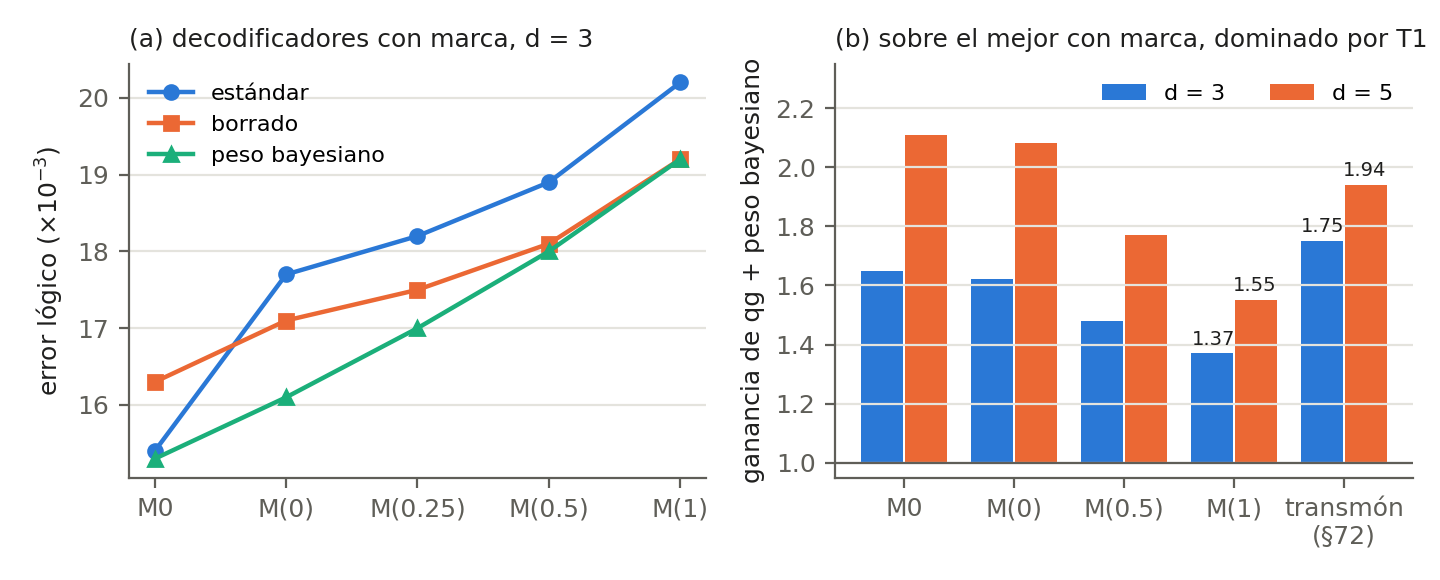
\includegraphics[width=\linewidth]{fig_leakage_es.png}
\caption{(a) Error lógico de los tres decodificadores con marca en los distintos modelos de fuga,
$d=3$, régimen dominado por T1. (b) Ganancia de qg + peso bayesiano sobre el mejor entre borrado y peso
bayesiano, a $d=3$ y $d=5$, incluido el canal del transmón de la Sección~\ref{sec:transmon}.}
\label{fig:leak}
\end{figure}

\subsection{Dónde queda un transmón}\label{sec:transmon}

Los parámetros de los modelos anteriores se eligieron, no se derivaron. Los derivamos para un transmón
a partir de una simulación coherente: dos transmones truncados a tres niveles (anarmonicidad
$-2\pi\cdot0{,}3$\,GHz, acoplamiento $2\pi\cdot10$\,MHz) y una CZ diabática por pulso de flujo a
través de la resonancia $|11\rangle\leftrightarrow|20\rangle$~\cite{dicarlo2009}, con el tiempo de
espera optimizado para la fidelidad de la compuerta tras correcciones Z virtuales. La compuerta llegó
a una fidelidad promedio de 0{,}99967, con fuga de $5{,}4\times10^{-4}$ desde $|11\rangle$ y exactamente
cero desde las demás entradas, así que $a=0$. Esto es estructural: el acoplamiento de intercambio
conserva el número de excitaciones y solo $|11\rangle$ puede llegar a $|20\rangle$. Un qubit de datos
fugado le da a su ancilla una fase condicional de $0{,}89\pi$, así que en un CNOT sigue invirtiéndola
con probabilidad $\kappa=0{,}97$, casi como si estuviera en $|1\rangle$; y decae de vuelta a $|1\rangle$
al doble de la tasa T1. El transmón fugado es casi invisible para sus estabilizadores y conserva su
valor: el rincón $M_0$ del mapa.

Con este canal en la memoria (y $|2\rangle$ leído como 1), se cumplieron las cuatro predicciones hechas
antes de la corrida (Tabla~\ref{tab:transmon}). El peso bayesiano empató con el estándar
(1{,}001$\times$, 1{,}011$\times$, 0{,}998$\times$; $|z|\le1{,}4$), el borrado perjudicó ($z=-7{,}2$,
$-4{,}9$, $-5{,}7$) y el decodificador qg sin marcas ganó 1{,}81$\times$ ($z=+15{,}3$) a $d=3$ y
2{,}02$\times$ ($z=+12{,}4$) a $d=5$. Agregarle la marca a qg costó un poco, porque el peso T1 del qubit
marcado se vuelve neutro aunque su bit sea correcto.

\begin{table}[t]
\centering\small
\caption{Error lógico con el canal de fuga derivado para una CZ de transmón, 60\,000 corridas por punto.}
\label{tab:transmon}
\begin{tabular}{clcccc}
\toprule
$d$ & régimen (testigo) & estándar & borrado & bayesiano & qg\\
\midrule
3 & dominado por T1 (1{,}68) & 0{,}0153 & 0{,}0163 & 0{,}0153 & 0{,}0084\\
3 & depolarizante (0{,}34) & 0{,}0031 & 0{,}0035 & 0{,}0030 & 0{,}0031\\
5 & dominado por T1 (2{,}30) & 0{,}0079 & 0{,}0084 & 0{,}0079 & 0{,}0039\\
\bottomrule
\end{tabular}
\end{table}

\subsection{Qubits de borrado}\label{sec:erasure}

Los qubits de borrado, como los transmones dual-rail~\cite{kubica2023erasure} y los átomos con
conversión de borrado~\cite{wu2022erasure}, anuncian los decaimientos en el momento en que ocurren.
Si el anuncio fuera perfecto, el sesgo de la lectura final que usa el decodificador qg no aportaría
nada más. Lo modelamos sobre la misma memoria, sin fuga: cada decaimiento $1\to0$ de un qubit de
datos se anuncia con probabilidad $h$ en su ubicación exacta, y el decodificador de borrado lleva esa
arista a probabilidad $1/2$.

La primera prueba predijo que la ganancia de qg + borrado sobre borrado caería con $h$ (cayó: de
1{,}59$\times$ y 2{,}04$\times$ con $h=0$ a menos de 1{,}1$\times$ con $h=0{,}99$) y que la combinación
nunca sería peor que el borrado solo. Esta última predicción falló, y la falla es el hallazgo: con
$h=0{,}99$, qg + borrado llegó apenas a 0{,}46$\times$ ($z=-6{,}7$) a $d=3$ y 0{,}22$\times$ a $d=5$.
La reponderación T1 supone que ningún decaimiento fue anunciado; con anuncios, un 0 en la lectura
final ya está mayormente explicado, y la reponderación lo cuenta dos veces. El testigo no lo detecta,
porque el sesgo de la lectura sigue presente para todo $h$.

Un arreglo exploratorio, encontrado después de esa corrida, escala la probabilidad previa de los
decaimientos \emph{no anunciados} por $1-h$ en ambos decodificadores. Después lo pusimos a prueba con
un registro previo nuevo: semillas nuevas, un segundo régimen (mixto), cinco valores de $h$ y un $h$
mal estimado en alrededor de 0{,}1. Se cumplieron las cuatro predicciones (Tabla~\ref{tab:erasure}).
Con la regla, qg + borrado nunca fue significativamente peor que el borrado calibrado (el punto más
cercano: 0{,}79$\times$, $z=-2{,}0$, régimen mixto, $d=5$, $h=0{,}9$); ganó 1{,}41$\times$ ($d=3$) y
1{,}68$\times$ ($d=5$) con $h=0{,}5$ y se desvaneció hasta cerca de 1 con $h=0{,}99$; la calibración
también mejoró al borrado solo con $h$ alto; y un error de 0{,}1 en $h$ cambió poco.

\begin{table}[t]
\centering\small
\caption{Ganancia de qg + borrado sobre borrado, ambos con la probabilidad previa de los decaimientos
no anunciados escalada por $1-h$ ($z$ apareado entre paréntesis), 60\,000 corridas por punto.}
\label{tab:erasure}
\setlength{\tabcolsep}{3.5pt}
\begin{tabular}{lcccccc}
\toprule
régimen & $d$ & $h=0{,}25$ & 0{,}5 & 0{,}75 & 0{,}9 & 0{,}99\\
\midrule
dominado por T1 & 3 & 1{,}50 (+11{,}1) & 1{,}41 (+9{,}0) & 1{,}25 (+4{,}2) & 1{,}09 (+1{,}2) & 0{,}92 ($-0{,}8$)\\
dominado por T1 & 5 & 1{,}93 (+9{,}0) & 1{,}68 (+5{,}4) & 1{,}39 (+2{,}8) & 1{,}45 (+2{,}2) & 1{,}00 (0{,}0)\\
mixto & 3 & 1{,}19 (+4{,}9) & 1{,}18 (+4{,}1) & 1{,}16 (+2{,}6) & 1{,}07 (+1{,}2) & 1{,}12 (+1{,}8)\\
mixto & 5 & 1{,}47 (+5{,}2) & 1{,}30 (+2{,}7) & 1{,}03 (+0{,}3) & 0{,}79 ($-2{,}0$) & 1{,}00 (0{,}0)\\
\bottomrule
\end{tabular}
\end{table}

\section{Qué lo decide}

Las seis pruebas encajan en un mismo cuadro. Que una lectura de tres niveles ayude depende de dos
propiedades del canal de fuga: la asimetría $a$, y si un qubit fugado conserva su valor mientras está
fugado. Cuando $a\approx0$ y el valor se conserva, como en la CZ de transmón simulada aquí, la marca no
aporta información nueva, el borrado descarta un bit correcto y la única ganancia es la reponderación
T1 a nivel de qubit. Cuando la fuga desordena el valor, la marca y la reponderación se complementan y
su ganancia crece con la distancia. El peso bayesiano de la Ec.~\eqref{eq:pflag} es una opción segura
por defecto en todo este rango, porque se reduce al decodificador estándar donde la marca no informa;
no es la mejor opción en todas partes. Para qang la conclusión es conservadora: las cantidades qg
siguen siendo cantidades de qubits, y una lectura de tres niveles entra, donde ayuda, como un dato más
para el decodificador qg, no como un qg nuevo. Los borrados anunciados son el límite en que la
información extra es completa: ahí hay que decirle a la reponderación qg cuánto ya se anunció, mediante
el escalado $1-h$, y se desvanece cuando $h\to1$.

\section{Limitaciones}

(i) Todo es simulación; no hay datos de hardware. (ii) Solo distancias 3 y 5, una tasa de fuga, fuga
solo después de los CNOT y sin unidades de reducción de fuga~\cite{mcewen2021leakage}. (iii) Los
modelos de fuga son clásicos; solo la compuerta de transmón de la Sección~\ref{sec:transmon} es
coherente, con un único pulso y conjunto de parámetros, truncamiento a tres niveles y una tasa de fuga
en la memoria cuatro veces mayor que la coherente, para tener estadística. El golpe a la pareja en el
evento de fuga y la asignación de $|2\rangle$ a 1 se suponen. (iv) El peso bayesiano supone que $a$ se
conoce por calibración y un prior uniforme sobre el valor previo a la fuga; una predicción sobre él
falló. (v) El modelo de borrado anuncia solo decaimientos de qubits de datos, en su ubicación exacta,
con $h$ conocido con un error de alrededor de 0{,}1. (vi) La decodificación por borrado y la detección de fuga son
conocidas~\cite{suchara2015leakage,wu2022erasure,varbanov2020leakage}; los aportes aquí son la prueba
del decodificador qg frente a ellas, el peso bayesiano con su prueba registrada de antemano, el
crecimiento de la ganancia combinada con la distancia y la ubicación de un transmón simulado en este
mapa, y la regla $1-h$ para combinar qg con borrados anunciados.

\section{Disponibilidad del código}
\sloppy
\texttt{examples/qutrit\_leakage\_qg.py}, \texttt{examples/qutrit\_leakage\_rounds\_qg.py},
\texttt{examples/qutrit\_bayes\_weight\_qg.py}, \texttt{examples/transmon\_leakage\_channel\_qg.py},
\texttt{examples/erasure\_qubits\_qg.py} y \texttt{examples/erasure\_calibrated\_qg.py}
en \url{https://github.com/Viny2030/qang} (licencia MIT), con tests de regresión. Las secciones 70 a 74
de \texttt{RESEARCH\_NOTES.md} dan más detalle.

\section*{Agradecimientos y uso de herramientas de IA}
Herramientas de IA generativa (Anthropic Claude Opus 5.5) asistieron con el código, los experimentos
numéricos, los tests y la redacción. El autor planteó las preguntas, tomó las decisiones de diseño y
revisó y validó todo el material asistido por IA, incluido cada número aquí reportado.

\bibliographystyle{unsrtnat}
\bibliography{../refs}
\end{document}
